\section{Regulator}
\label{sec:kontrollerdeign}
Det er valgt at designe regulatoren efter processen illustreret i figur \ref{fig:designproces}.
\begin{figure}[!th]
\centering
\include*{./graphics/designproces}
\caption[Designprocessen]{Designprocessen, \citep[Side. 260]{reg_modern_control_systems}.}
\label{fig:designproces}
\end{figure}

Formålet med reguleringen er som beskrevet i afsnit \ref{sec:problemformulering},
at kontrollere pan- og tilt-rammernes position, så de tracker en lerdue.
Dette gøres ved styring af deres hastighed, ved at justere spændingsfaldene over de
to DC-motorer. Spændingsfaldene styres af PWM-generatorer, og regulatoren
kan derfor styre motorernes hastighed ved at vælge PWM-signalernes duty cycles.

I afsnit \ref{sec:kravspecifikation} opstilles kravene til systemets respons.
Disse er for en 1-radian reference opsummeret nedenfor.
\begin{itemize}
\itemsep1pt
\item \(t_{s} \leq 0,557 \mathrm{\left[s\right]}\) (Settling Time)
\item \(SSE \leq 1,78 \%\) (Steady State Tracking Error)
\item \(P.O. \leq 34 \%\) (Overshoot i procent)
\end{itemize}

Det er fastlagt i projektoplægget, at regulatoren skal implementeres på mikrocontrolleren.
Da systemet som input modtager kartesiske koordinater,
skal der også på mikrocontrolleren foregå en koordinattransformation
til den logiske vinkelrepræsentation med sfæriske koordinater.
Systemets konfiguration består altså af en koordinattransformation,
en regulering, en aktuering og en positionsmåling, som illustreret
i figur \ref{fig:digitalkontroller1}.
Bemærk at denne konfiguration er for ét SISO-undersystem (enten pan eller tilt),
og at mikrocontrolleren skal regulere begge SISO-undersystemer.
\begin{figure}[!th]
\centering
\begin{tikzpicture}[auto, node distance=2.6cm,>=latex']
\include*{./graphics/digitalkontroller1}
\end{tikzpicture}
\caption[Systemkonfiguration]{Systemkonfiguration (blokdiagram).
	Området markeret med stiplet linje udgør den digitale regulator.
	De grønne ovaler angiver "clocksignaler", som leverer pulser til de digitale dele af systemet.}
\label{fig:digitalkontroller1}
\end{figure}
Som beskrevet i afsnit \ref{sec:problemformulering},
så er input-samplingen fastlagt til at foregå med en frekvens på 120 [Hz].
Men som illustreret på figur \ref{fig:digitalkontroller1}, så skal reguleringssløjfen
"køres" (sample) med en frekvens \(f_s=\frac{1}{T_s}\), der ikke nødvendigvis er 120 [Hz].
Dvs. A/D- og D/A-konverteringerne (ikke input-samplingen) skal foregå med frekvensen \(f_s\).

Der er overordnet to strategier til valg af samplingfrekvensen \(f_s\) hvormed
reguleringssløjfen skal køre:
1) Hvis man designer en kontinuert regulator til det kontinuerte domæne, så
skal diskretiseringen af controlleren være så tæt på den kontinuerte regulator som muligt.
Det vil sige, samplingfrekvensen skal vælges så høj som mulig.
2) Hvis man derimod designer en diskret regulator til det diskrete domæne,
så er diskretiseringen allerede foretaget inden designet af regulatoren.
Dvs. man finder en diskretiseret model af det fysiske system inden designet af regulatoren.
Kravet til diskretiseringen af åbensløjfeoverføringsfunktionerne er, at den diskrete repræsentation
skal være tilfredsstillende tæt på de kontinuerte overføringsfunktioner.
Hvis den diskrete overføringsfunktion eksempelvis afviger 20 \% fra den kontinuerte, ville man
sandsynligvis overveje at benytte en højere samplingfrekvens til diskretiseringen.
Sammenligningen af den diskrete overførselsfunktion og den kontinuerte overføringsfunktion
kan være både i tidsdomænet (fx steprespons) og i frekvensdomænet (frekvensrespons, fx. Bode-plots).
Når man har den diskretiserede model af systemet, kan man i det diskrete domæne (z-domænet)
udvikle en regulator - denne er altså diskret fra starten.

Da reguleringen foregår i en task på mikrocontrolleren, vælges det
at udvikle en diskret regulator efter en diskretiseret model af systemet.
Således kan perioden hvormed regulerings-task'en skal køre, fastlægges ud fra
samplingperioden \(T_s\). Hvis man havde valgt at designe en kontinuert regulator
ville perioden skulle vælges så lav som muligt, og dette ville stille højere krav
til mikrocontrolleren.

\subsection{Diskretisering af åbensløjfeoverføringsfunktionerne}
Som beskrevet ovenfor ønskes det at finde en diskretiseret overføringsfunktion
for det fysiske system. Den kontinuerte del af systemet, som ønskes diskretiseret,
er markeret på figur \ref{fig:digitalkontroller2}.
\begin{figure}[!th]
\centering
\begin{tikzpicture}[auto, node distance=2.6cm,>=latex']
\include*{./graphics/digitalkontroller2}
\end{tikzpicture}
\caption[Diskretisering af åbensløjfeoverføringsfunktion]{Diskretisering af åbensløjfdeoverføringsfunktion.
	Den kontinuerte del af systemet (markeret med stiplet linje) ønskes diskretiseret.
	De grønne ovaler angiver "clocksignaler", som leverer pulser til de digitale dele af systemet.}
\label{fig:digitalkontroller2}
\end{figure}

Den diskretiserede åbensløjfeoverføringsfunktion fra duty cycle til output vinkel
benævnes \(G_{zoh}\left(s\right)\). Dette er fordi D/A-konverteringen modelleres som et Zero-Order Hold kredsløb,
der fastholder en analog værdi proportional med duty cyclen. Dette stemmer overens med den simplificerede
model for PWM-signalet beskrevet i afsnit \ref{subsec:matFPGA}.
Den diskrete overføringsfunktions plads i blokdiagrammet for systemet
er indtegnet i figur \ref{fig:digitalkontroller3}.
\begin{figure}[!th]
\centering
\begin{tikzpicture}[auto, node distance=2.6cm,>=latex']
\include*{./graphics/digitalkontroller3}
\end{tikzpicture}
\caption[tekst i indholdsfortegnelsen]{figurtekst}
\label{fig:digitalkontroller3}
\end{figure}
De to overføringsfunktioner hhv. \(G_{pan}\left(s\right)\) og \(G_{tilt}\left(s\right)\)
har hver en diskretiseret overføringsfunktion hhv. \(G_{zoh,pan}\left(z\right)\) og \(G_{zoh,tilt}\left(z\right)\).

Kravet til \(G_{zoh,pan}\left(z\right)\) og \(G_{zoh,tilt}\left(z\right)\) er, at de
med god tilnærmelse opfører sig som \(G_{pan}\left(s\right)\) og \(G_{tilt}\left(s\right)\),
og dette krav kan skrives som et mindstekrav til samplingfrekvensen \(f_s\).

\subsubsection{Valg af samplingfrekvens}
\label{subsec:choosefs}
Reguleringssløjfen skal køre periodisk på mikroprocessoren
med samplingfrekvensen \(f_s\). Denne skal vælges
ud fra systemets dynamik (til diskretiseringen), som beskrevet ovenfor,
fra samplingteoremet (Nyquist-frekvensen) samt ud fra
mikrocontrollerens begrænsninger.

Da samplingen af inputparablen (A/D-konverteringen) foregår fast ved 120 [Hz],
som beskrevet i problemformuleringen, er rekonstruktionen
af det oprindelige signal allerede her begrænset. Dvs. man
ikke kan få mere information om det oprindelige signal
uanset hvor hurtigt man sampler efter A/D-konverteringen af
det oprindelige signal.
Samplingfrekvensen på 120 [Hz] fortæller os,
at det oprindelige signal kun er bevaret op til 60 [Hz].
Hvis reguleringssløjfen køres med en frekvens på under 120 [Hz]
vil \textit{mere} information gå tabt.
Derfor skal reguleringssløjfen, ud fra samplingteoremet, helst køres
ved minimum 120 [Hz].

Diskretiseringen af åbensløjfeoverføringsfunktionerne stiller også krav til samplingfrekvensen.
Diskretiseringen skal altså sammenlignes med den kontinuerte overføringsfunktion.
Det vælges at sammenligne diskretiseringen af det fysiske system med det kontinuerte system i tidsdomænet.
Sløjfen lukkes med en forstærkning på 1, og step-responsens karakteristik sammenlignes
for den diskretiserede overføringsfunktion \(\frac{G_{zoh,tilt}}{1+G_{zoh,tilt}}\)
og for den kontinuerte overføringsfunktion \(\frac{G_{tilt}}{1+G_{tilt}}\) (en tilsvarende sammenligning foretages for pan).
Diskretiseringen opfører sig med bedste tilnærmelse som det kontinuerte system
når Rise Time, Settling Time og Overshoot efter diskretiseringen
ændrer sig så lidt som muligt i forhold til responsen af det kontinuerte system.
Det vurderes, at Rise Time og Settling Time maks. må ændre sig med 5 \% i forhold
til den kontinuerte respons, mens at Overshoot maks. må ændre sig med 25 \% i forhold til
den kontinuerte respons.
Dvs. det kan tolereres hvis overshoot
ved diskretiseringen ændrer sig fra 2 \% til 3 \%.

Hvis diskretiseringen kræver at reguleringssløjfen kører ved en frekvens \(f_s\),
der er højere end A/D-konverteringens 120 [Hz], skal det A/D-konverterede
signal "upsamples" til \(f_s\).
Upsamplingen har den simpleste implementering
hvis \(f_s\) er et heltalsmultiplum af den første samplings frekvens (120 [Hz]) \citep[s. 562]{dsp}.
Diskretiseringen af det fysiske systems åbensløjfeoverføringsfunktioner skal altså samples ved et heltalsmultiplum \(f_s\) af 120 [Hz].

På figur \ref{fig:diskretTiltStep} er stepresponsen for lukketsløjfesystemet (med forstærkning 1)
med \(G_{tilt}\) indtegnet sammen med den tilsvarende steprespons for to forskellige diskretiseringer
af \(G_{tilt}\). Som det ses af grafen, er det diskretiserede systems respons tættest
på det kontinuerte systems respons når samplingfrekvensen er højest.
\begin{figure}[!th]
\centering
	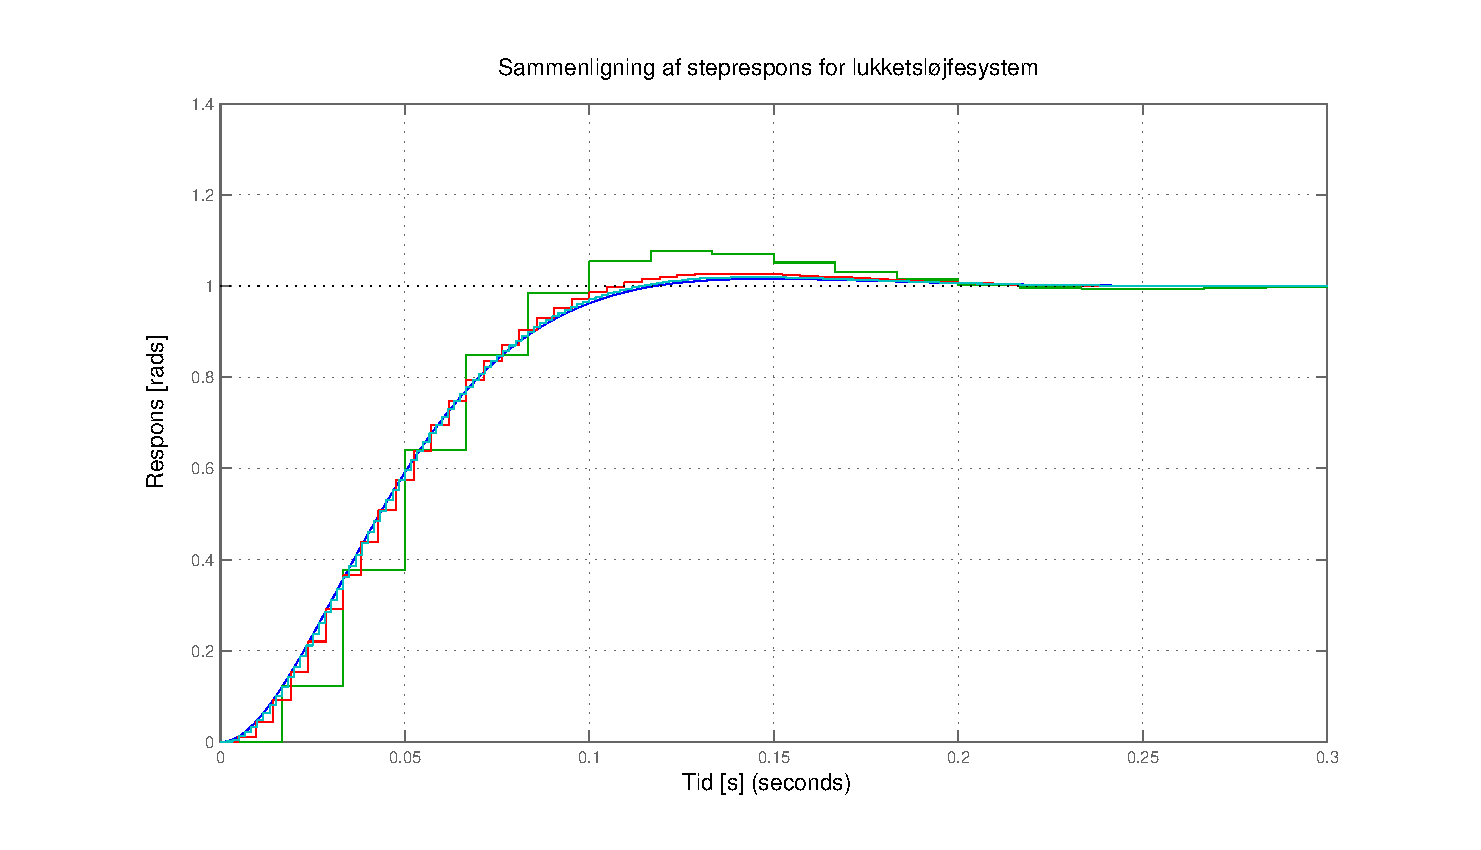
\includegraphics[width=1\textwidth]{./graphics/diskretTiltStep.eps}
\caption[Sammenligning af steprespons for kontinuert system med diskretiseret system]
{Sammenligning af steprespons for kontinuert system med diskretiseret system.
Den mørkeblå kurve er det kontinuerte systems respons,
og de andre kurver er det diskretiserede systems respons ved en samplingfrekvens på
120 [Hz] (grøn), 240 [Hz] (rød) og 600 [Hz] (lyseblå).}
\label{fig:diskretTiltStep}
\end{figure}
På figur \ref{fig:diskretStepFreq} er samme steprespons' performance afbildet
for pan og for tilt som funktion af samplingfrekvensen \(f_s\).
De sammenlignede størrelser er Rise Time, Settling Time og Overshoot.
Graferne viser ændringen af de tre størrelser i procent i forhold til det kontinuerte systems respons.
\begin{figure}[!th]
\centering
	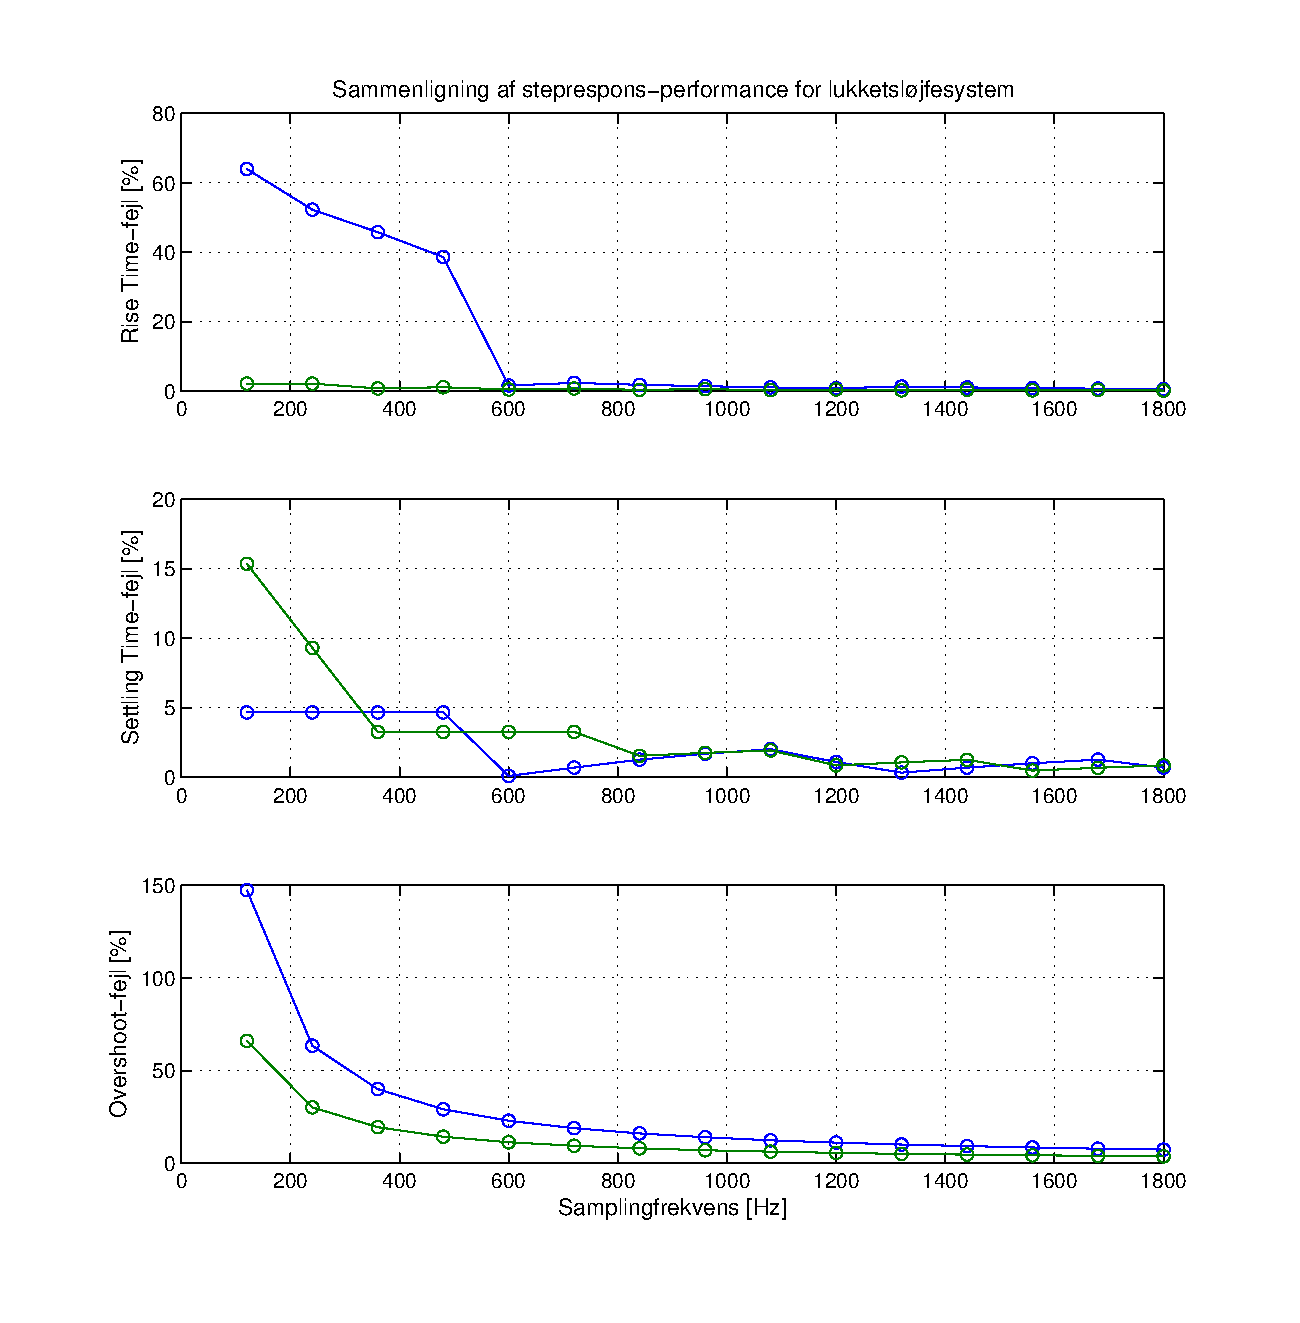
\includegraphics[width=1\textwidth]{./graphics/diskretStepFreq.eps}
%\caption[Sammenligning af steprespons-performance for kontinuert system med diskretiseret system (\(G_{zoh}\))]
%{Sammenligning af steprespons-performance for kontinuert system med diskretiseret system.
%Den blå kurve angiver fejlen i forhold til lukketsløjferesponsen af \(G_{tilt}\),
%mens den grønne kurve angiver fejlen i forhold til lukketsløjferesponsen af \(G_{pan}\).
%}

\caption[Sammenligning af steprespons-performance for kontinuert system med diskretiseret system $G_{zoh}$]
{Sammenligning af steprespons-performance for kontinuert system med diskretiseret system.
Den blå kurve angiver fejlen i forhold til lukketsløjferesponsen af $G_{tilt}$,
mens den grønne kurve angiver fejlen i forhold til lukketsløjferesponsen af $G_{pan}$.
}

% Åses LateX kan ikke lide \math\ i todo, caption og tilsvarende.

\label{fig:diskretStepFreq}
\end{figure}

Som forventet kan et generelt mønster ses på graferne i figur \ref{fig:diskretTiltStep} og figur \ref{fig:diskretStepFreq}:
Jo højere samplingfrekvens, jo tættere kommer diskretiseringens respons på det kontinuerte systems respons.
En yderligere inspicering viser, at en særligt god performance opnås ved en samplingfrekvens på 600 [Hz],
hvor kravene til diskretiseringens performance opfyldes.

Figur \ref{fig:diskretTiltStep} og figur \ref{fig:diskretStepFreq}
giver et grundlag for valg af reguleringssløjfens samplingfrekvens ud fra det fysiske systems dynamik.
Hvis mikrocontrollerens begrænsninger tages med i betragtning vil man vælge den lavest acceptable
samplingfrekvens af to årsager. Den ene årsag er, at jo højere periode, jo mindre CPU-belastning er der,
og jo mere tid er der til mikrocontrollerens andre opgaver som fx kommunikation med en PC-terminal.
Den anden årsag er, at reguleringssløjfen får mere tid til sine egne opgaver:
Koordinattransformation, upsampling, regulering (behandling af fejlsignalet) og SPI-kommunikation skal alt sammen foregå
inden for perioden \(\frac{1}{f_s}\).

Som udgangspunkt vælges derfor en samplingfrekvens på \(f_s=600 \mathrm{\left[Hz\right]}\),
så diskretiseringen med god tilnærmelse har samme performance som det kontinuerte system,
og så der er mest tid til reguleringssløjfens beregninger og SPI-kommunikation.

\subsubsection{Analyse af den diskretiserede overføringsfunktion}
I ligningerne \ref{eq:transpantilt1} findes de diskretiserede overføringsfunktioner.
\begin{align}
\label{eq:transpantilt1}
\begin{split}
	G_{zoh,pan}\left(z\right)&\approx\frac{7,94\cdot{}10^{-4}\cdot{}z^2
							+1,56\cdot{}10^{-3}\cdot{}z
							+1,18\cdot{}10^{-4}}
							{z^3 - 1,95\cdot{}z^2+9,67\cdot{}10^{-1}\cdot{z}-1,76\cdot{}10^{-2}}
	\\
	\\
	G_{zoh,tilt}\left(z\right)&\approx\frac{1,04\cdot{}10^{-3}\cdot{}z^2
							+2,03\cdot{}10^{-3}\cdot{}z
							+1,54\cdot{}10^{-4}}
							{z^3 - 1,93\cdot{}z^2+9,47\cdot{}10^{-1}\cdot{z}-1,76\cdot{}10^{-2}}
\end{split}
\end{align}
 
Den i afsnit \ref{subsec:choosefs} udførte sammenligning af det diskretiserede systems performance
med det kontinuerte systems performance viser,
at Rise Time stiger med 3,3 \% for pan og 0,10 \% for tilt,
Settling Time stiger med 0,48 \% for pan og 1,6 \% for tilt,
samt at Overshoot stiger med 11 \% for pan og 23 \% for tilt
ved lukketsløjfesystemet med en forstærkning på 1.
Diskretiseringen sammenlignes i frekvensdomænet med det kontinuerte system
i figur \ref{fig:diskretBode}, der viser Bode-plot for \(G_{pan}\) og \(G_{tilt}\) samt
deres diskretiseringer (ved 600 [Hz]) \(G_{zoh,pan}\) og \(G_{zoh,tilt}\).
\begin{figure}[!th]
\centering
	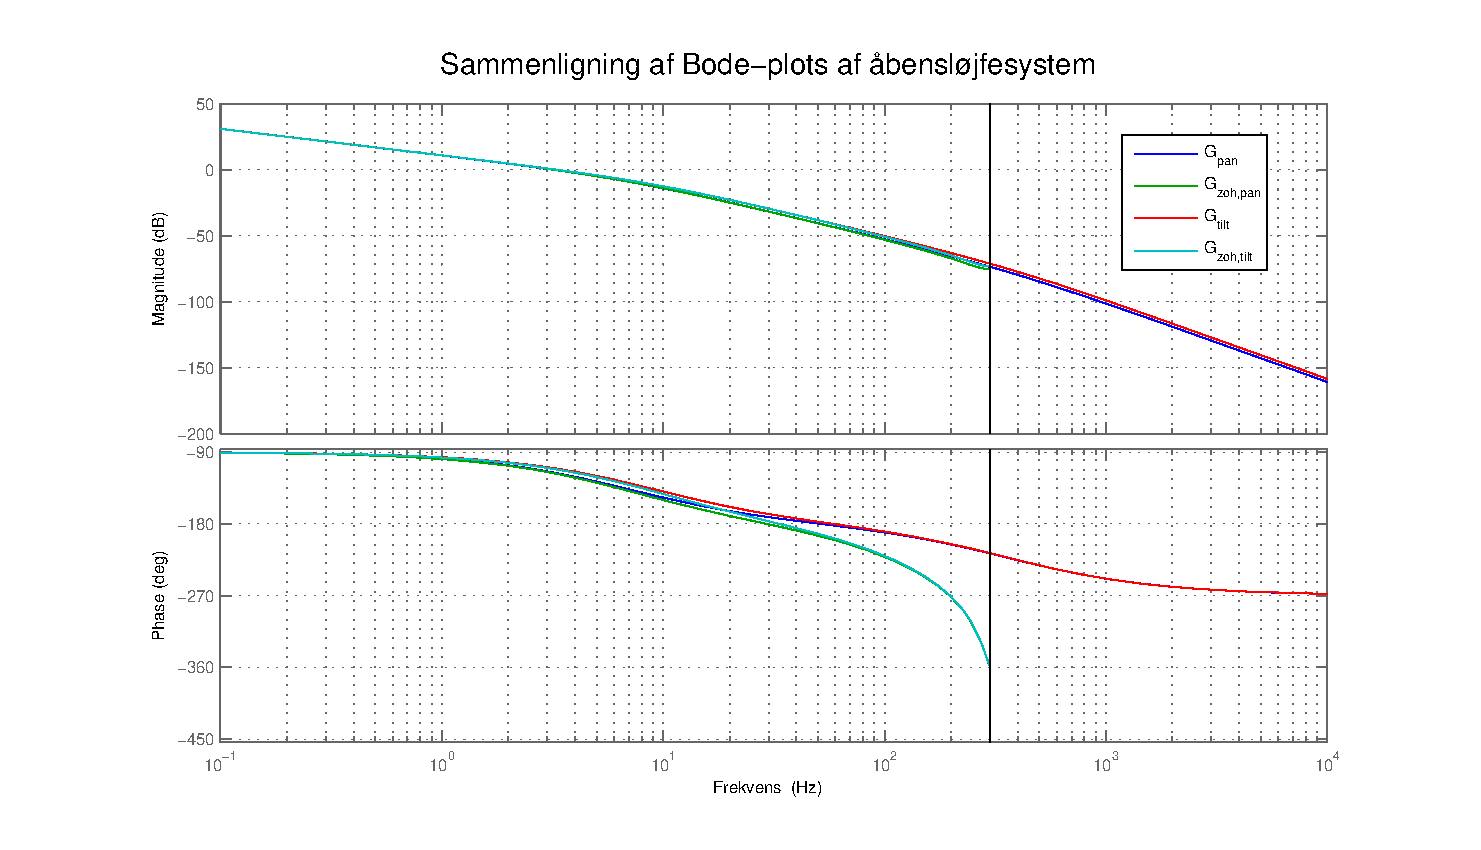
\includegraphics[width=1\textwidth]{./graphics/diskretBode.eps}
\caption[Sammenligning af Bode-plots af kontinuert system med diskretiseret system]
{Sammenligning af Bode-plots af kontinuert system med diskretiseret system.
Den blå og den røde kurve angiver hhv. \(G_{pan}\) og \(G_{tilt}\) mens
den grønne og den turkise kurve angiver hhv. \(G_{zoh,pan}\) og \(G_{zoh,tilt}\).
}
\label{fig:diskretBode}
\end{figure}
Bemærk at figur \ref{fig:diskretBode} er en sammenligning af \textit{åben}sløjfeoverføringsfunktionernes
frekvensrespons.

Som det ses på grafen, følger det diskretiserede systems respons meget nøje det kontinuerte systems respons.
Fejlen på størrelsen på responsen er meget lille i hele spektret,
mens fejlen på fasen er lille ved lave frekvenser og stiger ved høje frekvenser.

\subsection{Upsampling}
Da reguleringssløjfen, som beskrevet i afsnit \ref{subsec:choosefs}, køres med en frekvens på 600 [Hz],
som er 5 gange højere end input-samplingfrekvensen, skal der altså foretages en upsampling.
Upsamplingen foretages med Zero Order Hold, hvorved ét sample ved 120 Hz indsættes 
som 5 samples ved 600 Hz.
%Upsamplingen indsætter mellem hvert input-sample 4 samples med værdien 0, så hvert input-sample
%kun samples én gang. Dette gør, at input-signalets frekvensspektrum bevares.
Da input-signalet er samplet ved 120 [Hz] vil det oprindelige spektrum, centreret omkring 0 [Hz],
spejles ved heltalsmultipla af 120 [Hz]. Disse spejlbilleder af det oprindelige spektrum vil være
indeholdt i det upsamplede signal, hvis det ikke filtreres. 
En filtrering vil dog give signalet en forsinkelse før det når regulatoren,
og dette bidrager til fejlen. Det vælges derfor ikke at anvende et 
upsampling-filter.

\subsection{Valg af regulatortype}
Pga. de simplificerende antagler som er indeholdt i den matematiske model for systemet,
vil en åbensløjferegulering være et dårligt valg: den ville være følsom overfor afvigelser fra den
matematiske model. Desuden er der fra projektoplægget krav om en lukketsløjferegulering.
Den simpleste regulering ville være en konstant forstærkning af fejlsignalet.
En integrering af fejlsignalet ville gøre, at fejlsignalet ville blive tvunget mod 0,
og dette er ønsket ift. kravet om en tracking fejl på under 1,02 \degree.\todo[inline,author=Mikael]{Pythagoras! Come on guys!}
De største krav stilles til systemets responstid og ikke så meget til udsvinget af responsen,
og som udgangspunkt vælges derfor en PI-regulator, som gruppen er bekendt med fra
undervisningen i reguleringsteknik.

For at integratoren hurtigst muligt kan levere den nødvendige PWM-duty cycle til minimering af fejlsignalet,
vælges det desuden at implementere et "bias", der tager højde for dødbåndet.
Enhver PWM-duty cycle til Pan under 10 \% og til Tilt under 12 \%, og forskellig fra 0, bliver sat til hhv. 10 \% og 12 \%,
så Pan \& Tilt-systemet bevæger sig. For at undgå vedblivende svingninger vælges det desuden at nulstille
PWM-duty cycles under 1 \%.\todo[inline,author=Mikael]{Hvorfor 1 \%???}